\documentclass{article}
\usepackage{ctex}
\usepackage[a4paper, left=2.5cm, right=2.5cm, top=2.54cm, bottom=2.54cm]{geometry}
\usepackage{graphicx}
\usepackage{caption}
\usepackage{subcaption}
\usepackage{multirow}
\usepackage{multicol}
\usepackage{booktabs}
\usepackage[normalem]{ulem}
\usepackage{eqparbox}
\usepackage{listings}
\usepackage{mdframed}
\usepackage{amsmath}
\usepackage{enumerate}
\usepackage{placeins}
\usepackage{float}
\usepackage[dvipsnames]{xcolor}  % 使用 xcolor 包的 dvipsnames 选项
\usepackage[table,xcdraw]{xcolor}
% \usepackage{minted}
\useunder{\uline}{\ul}{}
\definecolor{code_bgc}{RGB}{255, 253, 253}  % 定义一个非常淡的粉色
\lstset{
    numbers=left,                   % 在左侧显示行号
    numberstyle=\color{Lavender},  % 设置行号的样式
    % frame=single,                   % 添加框架
    rulecolor=\color{black},        % 设置框架的颜色
    tabsize=2,                      % 设置tab的宽度
    breaklines=true,                % 自动折行
    breakatwhitespace=false,        % 在空白处折行
    escapeinside={\%*}{*)},         % 如果你想在代码中添加LaTeX代码,可以在此处设置
    keywordstyle=\color{RedViolet},      % 设置关键字的颜色
    commentstyle=\color{Salmon},   % 设置注释的颜色
    stringstyle=\color{RoyalBlue},      % 设置字符串的颜色
    basicstyle=\footnotesize,       % 设置代码的字体大小
    columns=fullflexible, 
    xleftmargin=2em,                % 设置左边距
    backgroundcolor=\color{code_bgc}, % 设置背景颜色
}
\newenvironment{codedisplay}[2]
{
    \begin{multicols}{3}
        \lstinputlisting[language={#1}]{#2}
    \end{multicols}
    
}

\begin{document}

\begin{table}
    \begin{tabular}{clllll}
    \multicolumn{4}{c}{\multirow{3}{*}{
\includegraphics[width=4.5cm]{assets/image.png}
    \fontsize{30}{35}\selectfont\kaishu 实验报告}}            & \quad 专业: & {\ul{\eqparbox{col4}{\quad 电子信息工程 \quad}}}     \\
    \multicolumn{4}{c}{}                                      & \quad 姓名: & {\ul {\eqparbox{col4}{\qquad 冯静怡}}}        \\
    \multicolumn{4}{c}{}                                      & \quad 学号: & {\ul {\eqparbox{col4}{\quad 3220104119}}} \\
    课程名称: & {\ul {\eqparbox{col1}{\quad 微机原理及应用\quad}}} & \quad 指导老师:    & {\ul {\eqparbox{col2}{吴建德、胡斯登\quad}}} 
     & \quad 地点: & {\ul {\eqparbox{col4}{ 紫金港东三406}}}   \\
    实验名称: & {\ul {\eqparbox{col1}{\quad 旋转钟\quad }}}       &\quad & {\ul}
    &\quad 日期: & {\ul {\eqparbox{col4}{\today}}}      
    \end{tabular}
    \end{table}

\section{实验目的}
\begin{enumerate}
    \item 熟练使用STM32的C语言编程。
    \item 熟悉STM32的定时器和中断方式。
    \item 学会软硬件协同设计。
\end{enumerate}
\section{实验过程}
\subsection{实验基本完成功能}
\begin{enumerate}
    \item \textbf{文字显示:}旋转钟侧面显示“姓名、学号”,并能够进行滚动。
    \item \textbf{时钟显示:}旋转钟正面显示时间,通过DS1302芯片,实时显示时间。
    \item \textbf{红外控制:}红外遥控对旋转钟的显示进行控制。
\end{enumerate}
\subsection{硬件功能分析}
\subsubsection{旋转灯供电}
通过type-C接口输入电源,随后通过线圈耦合,使得type-C中的电源输入到上面的面板,从而实现STM32的供电。
\subsubsection{74HC595功能介绍与分配}
\begin{figure}[H]
\begin{minipage}{0.5\textwidth}
    \centering
    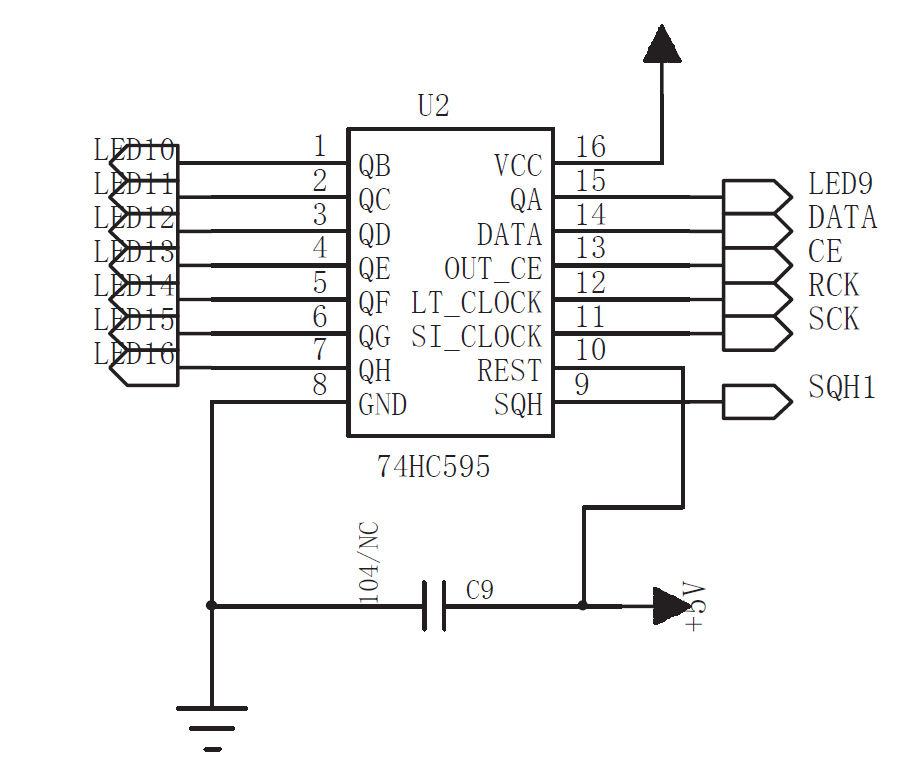
\includegraphics[width=0.8\linewidth]{assets/1.png}
    \caption{74HC595硬件框图}
    \label{fig:hard}
\end{minipage}
\begin{minipage}{0.5\textwidth}
\ \ \ \ \ \ 595芯片实现了通过1个串行引脚、1个时钟同步控制信号和1个使能端,控制8个输出,以扩展STM32本身芯片的功能。\par
\ \ \ \ \ \ 通过SQH引脚,输入到下一个引脚的DATA之中,从而实现多片595串联,从而可以通过1个DATA引脚控制(本实验中)32个引脚的输出。\par
\end{minipage}
\end{figure}
\begin{figure}[H]
    \begin{minipage}{0.69\textwidth}
\ \ \ \ \ \ 595芯片主要由3部分组成:移位寄存器,8位寄存器,输出\par
\ \ \ \ \ \ $\texttt{RCK}$(图中$\texttt{SH\_CP}$)为移位寄存器信号,每一个上升沿将$\texttt{DATA}$中的数据输入到移位寄存器中,并进行移位。\par
\ \ \ \ \ \ $\texttt{SCK}$(图中$\texttt{ST\_CP}$)为8位寄存器信号,每一个上升沿将移位寄存器的数据存储到8位寄存器,并输出。\par
\ \ \ \ \ \ $\overline{\texttt{OE}}$控制输出使能,高为禁止输出态,输出高阻态,本实验中直接设置其为低电平,保证能够实时显示LED灯亮。\par
    \end{minipage}
    \begin{minipage}{0.3\textwidth}
        \centering
        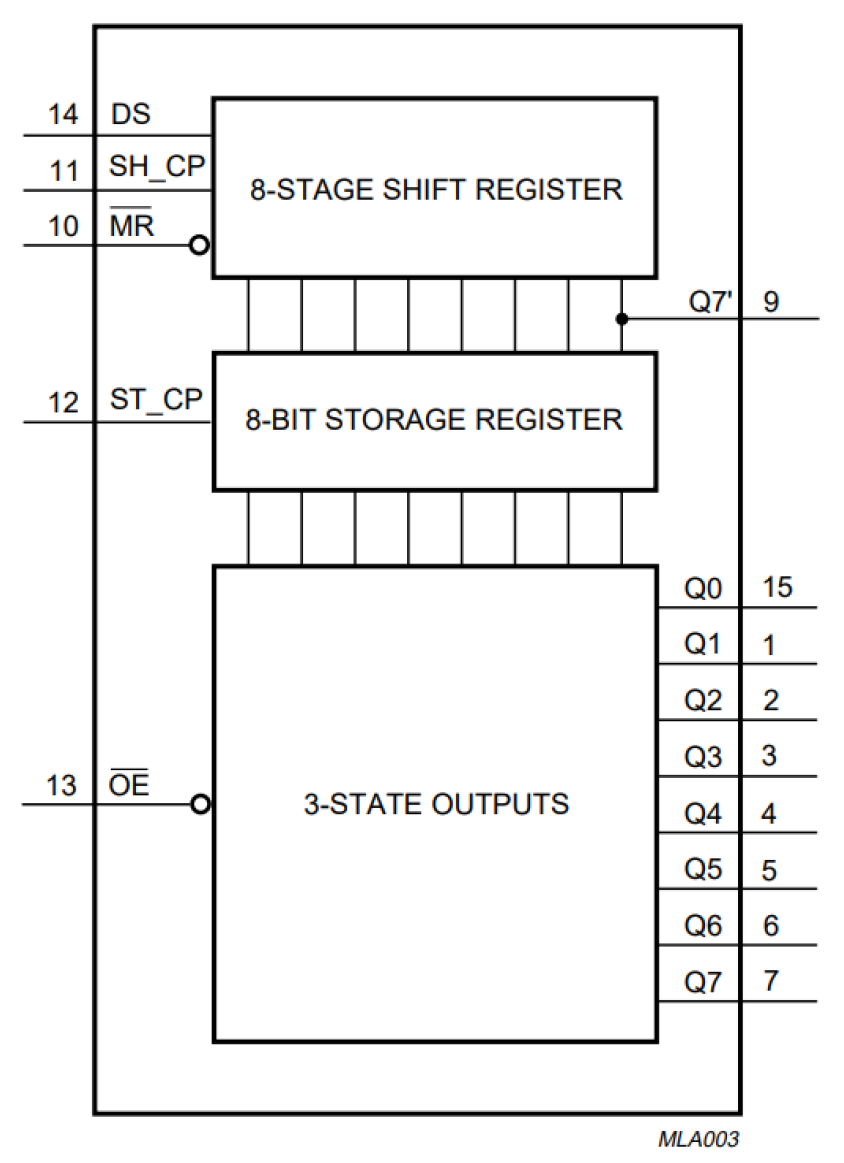
\includegraphics[width=0.8\linewidth]{assets/2.png}
        \caption{595芯片内部原理}
    \end{minipage}
\end{figure}
595芯片控制32盏灯的控制代码:
\begin{multicols}{2}
\begin{lstlisting}[language=c]
shine = LED_Data;
tmp = 0x80000000;   //shine的掩码,代表当前处理的位,先处理最高位。
LL_GPIO_ResetOutputPin(SCK_GPIO_Port, SCK_Pin); //shift Register置低,准备迎接上升沿
LL_GPIO_ResetOutputPin(RCK_GPIO_Port, RCK_Pin); //8-bit Register置低,准备迎接上升沿
for(int i=0;i<32;i++)
{
    if(shine & tmp) //如果当前位要亮
        LL_GPIO_ResetOutputPin(DATA_GPIO_Port, DATA_Pin);   //DATA置0代表亮灯
    else
        LL_GPIO_SetOutputPin(DATA_GPIO_Port, DATA_Pin);
    Delay;
    LL_GPIO_SetOutputPin(SCK_GPIO_Port, SCK_Pin);   //移位寄存器创造一个上升沿,将DATA数据输入
    Delay;
    LL_GPIO_ResetOutputPin(SCK_GPIO_Port, SCK_Pin); //置低,准备迎接上升沿
    tmp = tmp >> 1;
}
LL_GPIO_SetOutputPin(RCK_GPIO_Port, RCK_Pin);   //上升沿,存储同时输出移位寄存器中的32位数据
Delay;
LL_GPIO_ResetOutputPin(RCK_GPIO_Port, RCK_Pin);
\end{lstlisting}
\end{multicols}
\subsubsection{LED灯显示}
\paragraph{LED灯排布}由于LED分布的特殊性,所以在编程过程中,需要注意对LED灯进行转换,使其正常输出。
\begin{multicols}{2}
\eqparbox{led}{\textbf{LED17-32}}\ 由STM32的GPIO直接控制。\par
\eqparbox{led}{\textbf{LED9-16}}\ $\texttt{DATA}$数据的0-7位;\par
\eqparbox{led}{\textbf{LED1-8}}\ $\texttt{DATA}$数据的8-15位;\par
\eqparbox{ledd}{\textbf{D1-8\ }}\ $\texttt{DATA}$数据的23-16位;\par
\eqparbox{ledd}{\textbf{D9-16}}\ $\texttt{DATA}$数据的31-24位;\par
\end{multicols}
\paragraph{数据显示}将旋转钟转一圈分为240份。
\begin{figure}[H]
\begin{minipage}{0.7\textwidth}
\ \ \ \ \ \ 旋转钟一圈的判定通过硬件中的红外发射/接收设备。
当红外停止接收红外信号,产生一个上升沿,
从而触发中断,记录两次中断间的时间,重新设置显示中断为中断时间的$1/240$,从而能够在每一个位置精确显示特定数值。
显示中断每次显示调用LED显示函数。
\end{minipage}
\begin{minipage}{0.29\textwidth}
    \centering
    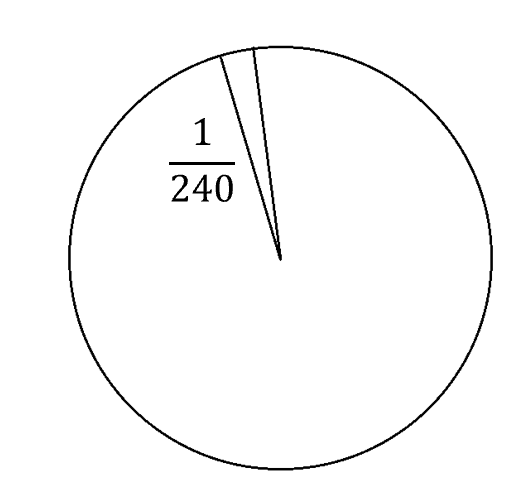
\includegraphics[width=0.6\linewidth]{assets/4.png}
    \caption{LED显示示意图}
\end{minipage}
\end{figure}
\subsubsection{DS1302芯片}
\begin{figure}[H]
    \begin{minipage}{0.49\textwidth}
        \centering
        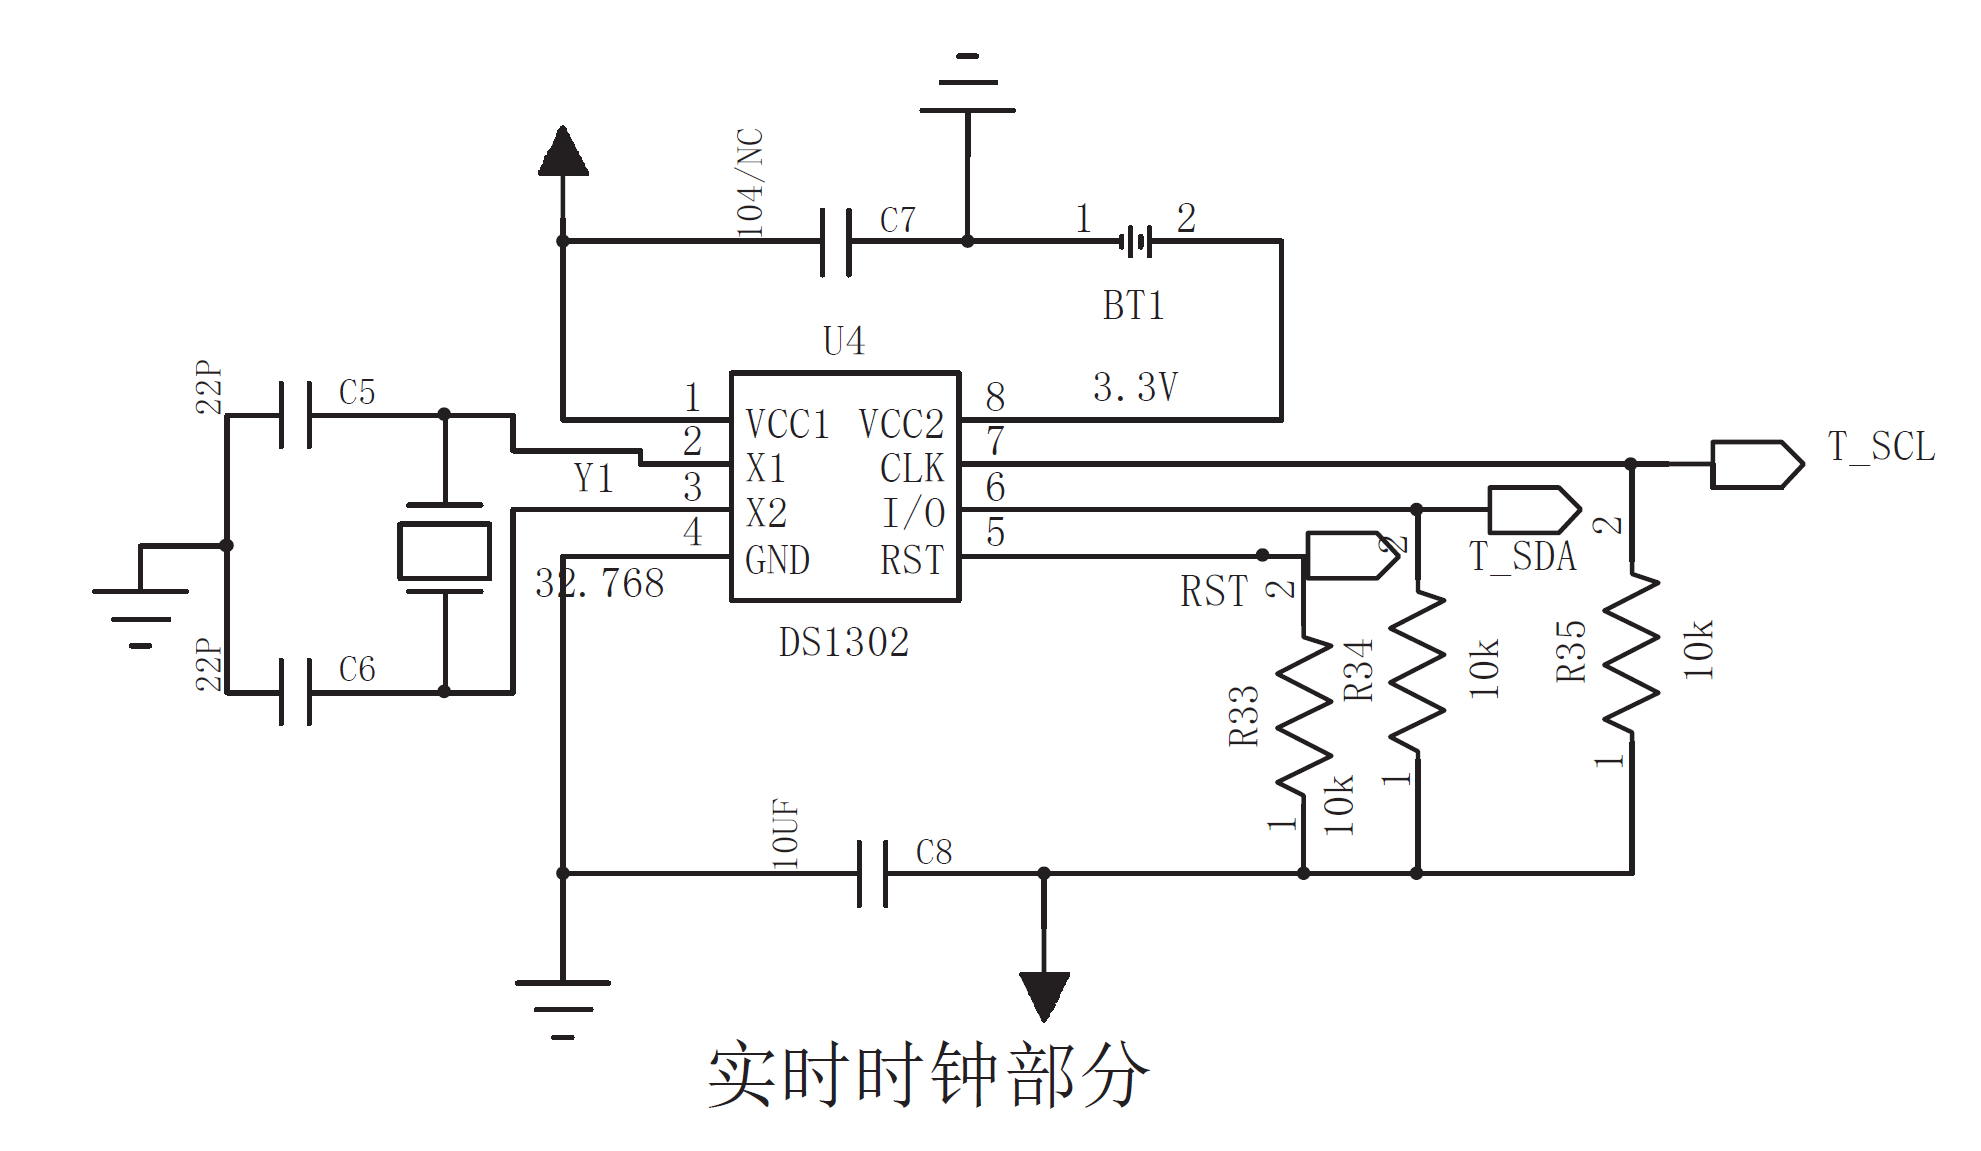
\includegraphics[width=0.99\linewidth]{assets/5.png}
        \caption{DS1302硬件框图}
    \end{minipage}
    \begin{minipage}{0.5\textwidth}
    \ \ \ \ \ \ DS1302 是DALLAS 公司推出的涓流充电时钟芯片内含有一个实时
    时钟/日历和31 字节静态RAM,可通过简单的串行接口与单片机进行通信。\par
    控制引脚有:
    \begin{itemize}
        \item $\texttt{T\_SCL}$同步时钟信号,方便IO口时序同步。
        \item $\texttt{T\_SDA}$串行数据输入/输出。
        \item $\texttt{RST}$为高则启用串行输入/输出。
    \end{itemize}
    \end{minipage}
\end{figure}
\paragraph{对DS1302进行读写操作}DS1302有可读写的寄存器,存储了时间信息。
\begin{figure}[H]
    \begin{subfigure}{0.5\textwidth}
        \centering
        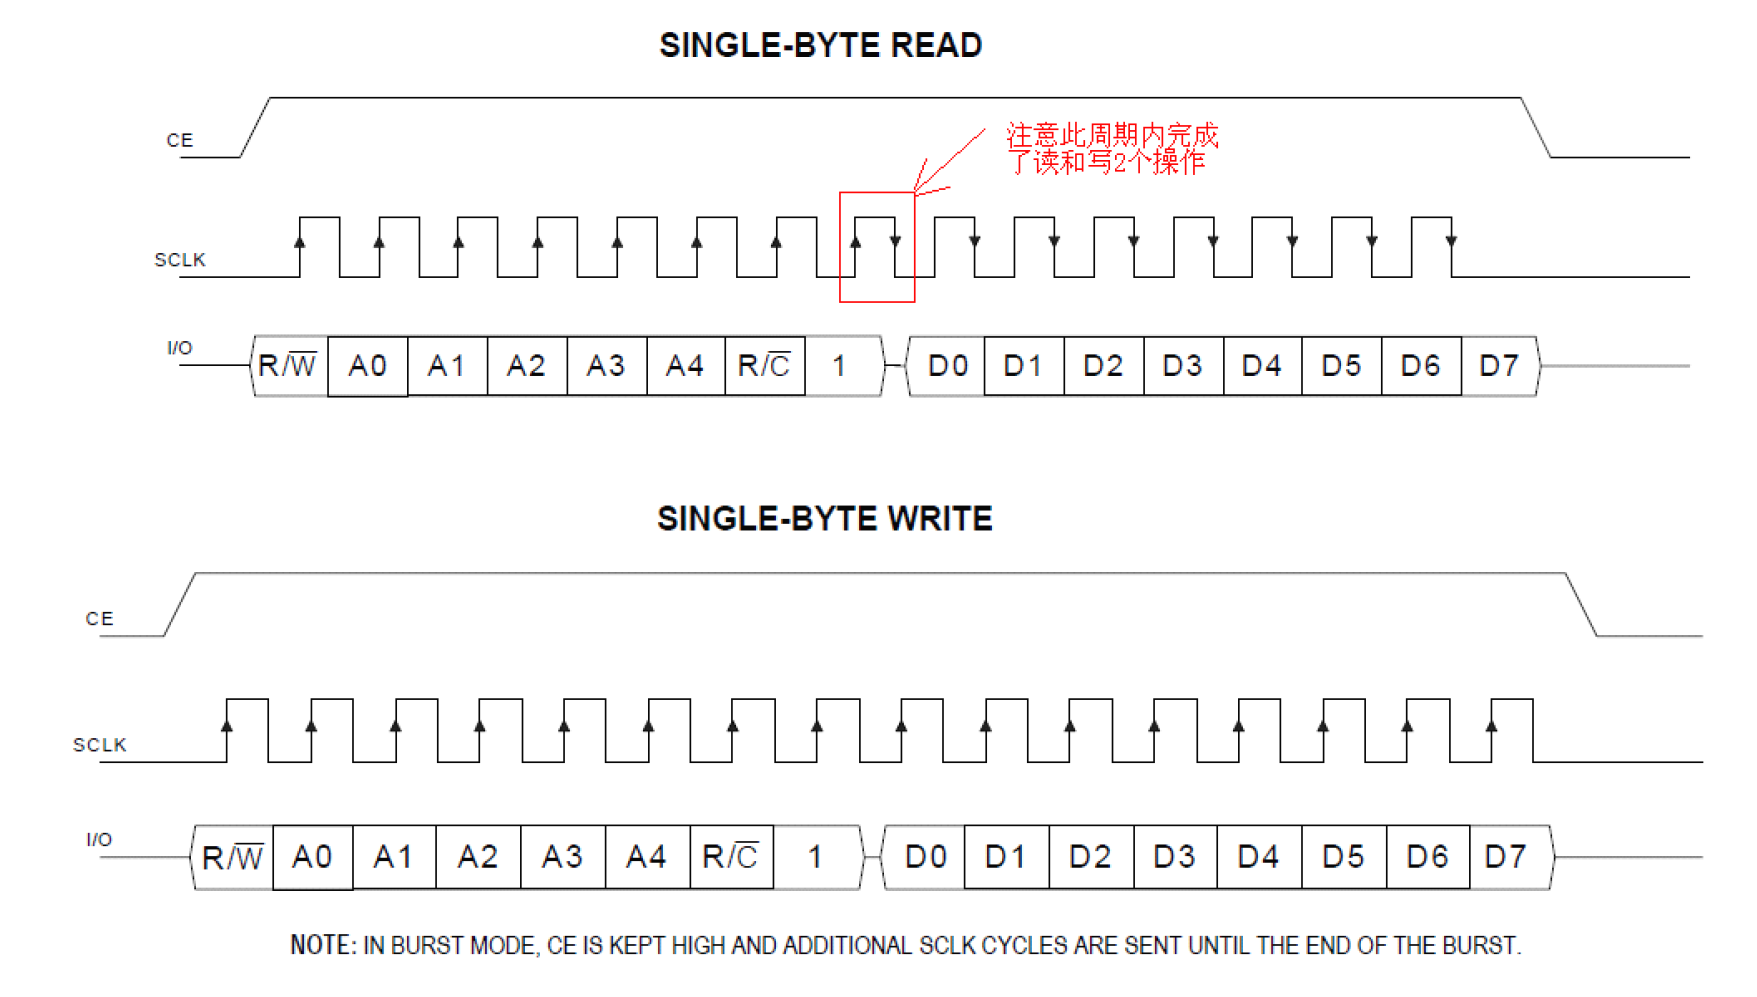
\includegraphics[width=0.99\linewidth]{assets/6.png}
        \caption{DS1302读写时序图}
    \end{subfigure}
    \begin{subfigure}{0.5\textwidth}
        \centering
        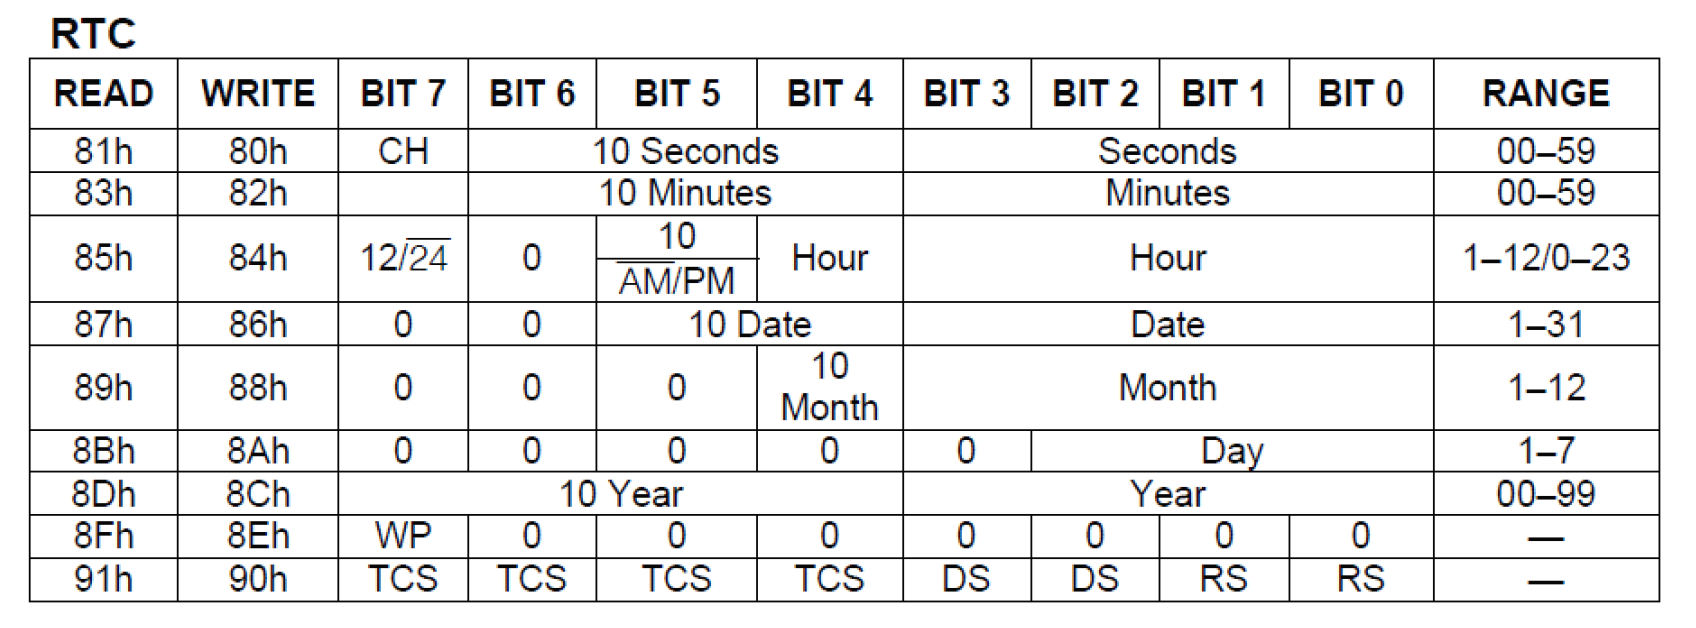
\includegraphics[width=0.99\linewidth]{assets/7.png}
        \caption{DS1302寄存器说明}
    \end{subfigure}
    \caption{DS1302读写操作}
\end{figure}
\paragraph{写入数据}写入数据时,命令由两部分组成,1. 寄存器地址;2. 寄存器要存放的8位数据\par
\begin{multicols}{2}
\begin{lstlisting}[language=c]
/*通过GPIO的Output模式模拟串行口输出数据*/
void DS1302WriteByte(uint8_t dat)
{
  uint8_t i;
  LL_GPIO_ResetOutputPin(T_SCL_GPIO_Port, T_SCL_Pin);
  for(int delay=0;delay<2;delay++){}
  for(i=0;i<8;i++)
  {
    if(dat&0x01)
      LL_GPIO_SetOutputPin(T_SDA_GPIO_Port, T_SDA_Pin);
    else
      LL_GPIO_ResetOutputPin(T_SDA_GPIO_Port, T_SDA_Pin);
    Delay;
    LL_GPIO_SetOutputPin(T_SCL_GPIO_Port, T_SCL_Pin);
    Delay;
    LL_GPIO_ResetOutputPin(T_SCL_GPIO_Port, T_SCL_Pin);
    dat>>=1;
  }
}
/* DS1302Write写入命令、数据,主要依靠 DS1302WriteByte 实现*/
void DS1302Write(uint8_t cmd, uint8_t dat)
{
    LL_GPIO_ResetOutputPin(RST_GPIO_Port, RST_Pin);
    LL_GPIO_ResetOutputPin(T_SCL_GPIO_Port, T_SCL_Pin);
    LL_GPIO_SetOutputPin(RST_GPIO_Port, RST_Pin);
    DS1302WriteByte(cmd);
    DS1302WriteByte(dat);
    LL_GPIO_SetOutputPin(T_SCL_GPIO_Port, T_SCL_Pin);
    LL_GPIO_ResetOutputPin(RST_GPIO_Port, RST_Pin);
}
\end{lstlisting}
\end{multicols}
\paragraph{读取数据}读入数据时,先要输入要读取数据的地址命令,然后调节GPIO模式为INPUT从而读入数据\par
\begin{multicols}{2}
\begin{lstlisting}[language=c]
/*通过GPIO的Input模式模拟串行口输入数据*/
uint8_t DS1302ReadByte(void)
{
  uint8_t i,dat=0;
  for(int delay=0;delay<1;delay++){}
  for(i=0;i<8;i++)
  {
    dat>>=1;
    if(LL_GPIO_IsInputPinSet(T_SDA_GPIO_Port, T_SDA_Pin))
      dat|=0x80;
    LL_GPIO_SetOutputPin(T_SCL_GPIO_Port, T_SCL_Pin);
    Delay;
    LL_GPIO_ResetOutputPin(T_SCL_GPIO_Port, T_SCL_Pin);
    Dealy;
  }
  return dat;
}
/* DS1302Read写入命令、数据,主要依靠 DS1302ReadByte/WriteByte 实现*/
uint8_t DS1302Read(uint8_t cmd)
{
  uint8_t dat=0;
  LL_GPIO_ResetOutputPin(RST_GPIO_Port, RST_Pin);
  LL_GPIO_ResetOutputPin(T_SCL_GPIO_Port, T_SCL_Pin);
  LL_GPIO_SetOutputPin(RST_GPIO_Port, RST_Pin);
  DS1302WriteByte(cmd);
  LL_GPIO_SetPinMode(T_SDA_GPIO_Port, T_SDA_Pin, LL_GPIO_MODE_INPUT);
  dat=DS1302ReadByte();
  LL_GPIO_SetPinMode(T_SDA_GPIO_Port,T_SDA_Pin,LL_GPIO_MODE_OUTPUT);
  LL_GPIO_SetOutputPin(T_SCL_GPIO_Port, T_SCL_Pin);
  LL_GPIO_ResetOutputPin(RST_GPIO_Port, RST_Pin);
  return dat;
}
\end{lstlisting}
\end{multicols}
\paragraph{DS1302初始化}在第一次使用DS1302时,需要对芯片内的数据进行初始化,具体代码如下:
\begin{multicols}{2}
\begin{lstlisting}[language=c]
void Init_DS1302(void)
{
    DS1302Write(0x8e, 0x00); // 控制寄存器地址 0x8E, 数据 0x00 (解除写保护)
    DS1302Write(0x80, 0x20); // 秒寄存器地址 0x80, 数据 0x20 (20秒)
    DS1302Write(0x82, 0x27); // 分钟寄存器地址 0x82, 数据 0x27 (27分钟)
    DS1302Write(0x84, 0x89); // 小时寄存器地址 0x84, 数据 0x89 (12小时制, 9点)
    /*年月日星期代码略*/
    DS1302Write(0x90, 0x01); // 充电寄存器地址 0x90, 数据 0x01 (启用充电)
    DS1302Write(0xc0, 0xf0); // RAM 地址 0xC0, 数据 0xF0 (初始化标志)
    DS1302Write(0x8e, 0x80); // 控制寄存器地址 0x8E, 数据 0x80 (启用写保护)
}
\end{lstlisting}
\end{multicols}
\paragraph{从DS1302芯片中读取实时数据}设置中断,每秒从DS1302中读取一次数据,就能够实现时间显示。
\begin{multicols}{2}
\begin{lstlisting}[language=c]
void getdate()
{
    // 读取年份
    date1 = DS1302Read(0x8D);
    date[0] = (date1 & 0xF0) >> 4; // 年高位
    date[1] = date1 & 0x0F;        // 年低位
    // 读取月份
    date1 = DS1302Read(0x89);
    date[2] = (date1 & 0xF0) >> 4; // 月高位
    date[3] = date1 & 0x0F;        // 月低位
    /*其余代码略*/
}
\end{lstlisting}
\end{multicols}
\subsubsection{红外遥控}
\paragraph{接收到红外信号终端控制}当接收到红外遥控信号,通过下降沿进行中断\par
以下代码用于通过外部中断处理程序,以读取红外信号的脉冲宽度,并根据脉冲宽度解码成对应的红外数据。
最终将解码得到的数据存储在 command 变量中。\par
\begin{multicols}{2}
\begin{lstlisting}[language=c]
if (LL_EXTI_IsActiveFlag_0_31(LL_EXTI_LINE_7) != RESET)
{
    LL_EXTI_ClearFlag_0_31(LL_EXTI_LINE_7);

    // 获取当前的定时器计数器值
    currentCapture = LL_TIM_GetCounter(TIM2);

    // 计算脉冲宽度
    pulseWidth = currentCapture - lastCapture;
    lastCapture = currentCapture;
    laaCapture = lastCapture;

    // 判断脉冲宽度,根据不同的条件进行处理
    if (pulseWidth > 13000 && pulseWidth < 14000 && dataReady == 0)  // 9000+4500 = 13500
    {
        // 开始读取数据,重置状态
        bitIndex = 0;
        command_pre = 0;
        FinishReading = 0;
    }
    else if (pulseWidth > 10500 && pulseWidth < 12000 && FinishReading != 1) // 9000+2250 = 11250
    {
        // 继续读取数据,重置状态
        bitIndex = 0;
        command_pre = 0;
    }
    else if (FinishReading)
    {
        // 数据已读取完成,退出
        return;
    }
    else if (pulseWidth < 500)
    {
        // 脉冲宽度太短,可能是干扰或者无效信号,忽略
        lastCapture = laaCapture;
        return;
    }
    else if (pulseWidth > 2000 && pulseWidth < 2500) // 560+1690 = 2250
    {
        // 长脉冲表示二进制位为1
        command_pre = (command_pre << 1) | 1;
        bitIndex++;
    }
    else if (pulseWidth > 800 && pulseWidth < 1500) // 560+560 = 1120
    {
        // 短脉冲表示二进制位为0
        command_pre = command_pre << 1;
        bitIndex++;
    }

    // 判断是否已经读取完32位数据
    if (bitIndex == 32)
    {
        // 数据已经完整读取
        bitIndex = 0;
        command = command_pre; // 将解码后的数据存入 command 变量
        dataReady = 1;          // 数据标志位,表示数据已准备好
        FinishReading = 1;      // 结束读取状态
    }
}
\end{lstlisting}
\end{multicols}
\paragraph{代码功能解释}
\begin{itemize}
    \item $\texttt{currentCapture = LL\_TIM\_GetCounter(TIM2)}$:获取定时器 TIM2 的当前计数值,以计算上一次实验到现在的时间。
    \item $\texttt{pulseWidth = currentCapture - lastCapture}$:计算当前脉冲的宽度。
    \item 信号判断:根据红外通信协议,长脉冲代表二进制位为1,短脉冲代表二进制位为0。
    \item \textbf{数据存储:}\par
    $\texttt{command\_pre}$ 变量存储正在解码的数据。\par
    $\texttt{command}$ 变量最终存储完整的解码数据。\par
    \item \textbf{状态标志位:}\par
    $\texttt{bitIndex}$ 记录当前位的索引。\par
    $\texttt{dataReady}$ 标志位表示数据已准备好。\par
    $\texttt{FinishReading}$ 标志位表示数据读取完成。\par
\end{itemize}
\paragraph{主程序}对读取到的红外数据进行处理,使用查询方法。
\begin{multicols}{2}
\begin{lstlisting}[language=c]
while (1)
{
    if (dataReady)
    {
        switch (command)
        {
            case IRR_Start:
                LL_GPIO_TogglePin(LED00_GPIO_Port, LED00_Pin);
                break;
            case IRR_Right:
            /*代码略*/  
            default:
                break;
        }
        dataReady = 0;
        /*避免红外信号冲突,延时0.5s*/
        LL_mDelay(500);
        FinishReading = 0;
    }
}
\end{lstlisting}
\end{multicols}
设置$\texttt{WorkState}$,在循环中根据case判断结果,在main.h中设置WorkState掩码,便于操作。
\begin{multicols}{3}
\begin{lstlisting}[language=c]
#define NEC_Rotate_Right (1<<0)
#define NEC_Rotate_Left (1<<1)
#define NEC_Time_Adjust (1<<2)
#define NEC_Show (1<<3)
\end{lstlisting}
\end{multicols}
\subsubsection{定时器}
\paragraph{TIM1}用于调用DS1302读取时间函数,每500ms调用一次。\par
\begin{figure}[H]
\begin{minipage}{0.5\textwidth}
    \centering
    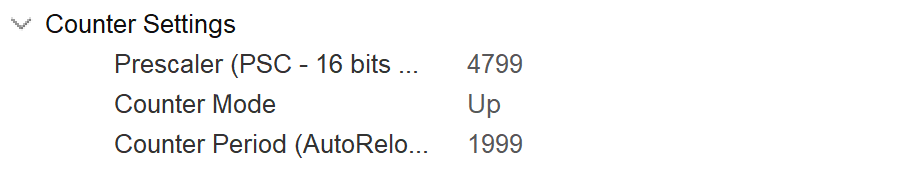
\includegraphics[width=0.9\linewidth]{assets/8.png}
    \caption{TIM1设置}
\end{minipage}
\begin{minipage}{0.49\textwidth}
    $$
    t=\frac1{48\cdot10^6}\cdot(4800-1)\cdot (2000-1)=0.5s
    $$
\end{minipage}
\end{figure}
中断函数代码如下:\par
\begin{multicols}{2}
\begin{lstlisting}
if(LL_TIM_IsActiveFlag_UPDATE(TIM1)!= RESET)
  {
    LL_TIM_ClearFlag_UPDATE(TIM1);
    getdate();  //读取DS1302时间
    spoint=date[12]*10+date[13];    //秒
    mpoint=date[10]*10+date[11];    //分
    hpoint=(date[8]&1)*10+date[9];  //时
  }
\end{lstlisting}
\end{multicols}
\paragraph{TIM2}设置us计时器,用于读取红外遥控信号,不设置中断。
\begin{figure}[H]
    \begin{minipage}{0.5\textwidth}
        \centering
        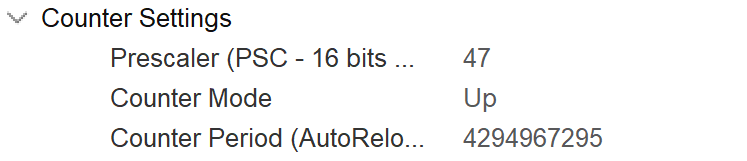
\includegraphics[width=0.9\linewidth]{assets/9.png}
        \caption{TIM2设置}
    \end{minipage}
    \begin{minipage}{0.49\textwidth}
        $$
        t=\frac1{48\cdot10^6}\cdot(48-1)=1us
        $$
    \end{minipage}
    \end{figure}
\paragraph{TIM3}用于LED显示,具体时间由红外读取中断内控制。\par
红外中断控制代码(GPIO下降沿中断):\par
\begin{multicols}{2}
\begin{lstlisting}[language=c]
if (LL_EXTI_IsActiveFlag_0_31(LL_EXTI_LINE_6) != RESET)
  {
    LL_EXTI_ClearFlag_0_31(LL_EXTI_LINE_6);
    /* USER CODE BEGIN LL_EXTI_LINE_6 */
    if(timecount<120) return; //防止误触发
    //获取TIM3当前counter值以及autoreload重复次数,以便计算240份情况下应该的autoreload值。
    uint16_t timeint = (timecount*(LL_TIM_GetAutoReload(TIM3)+1)+LL_TIM_GetCounter(TIM3)+1)/240;
	LL_TIM_SetAutoReload(TIM3,timeint-1);
    timecount = 0;  //在TIM3中累加,此处清零
  }
\end{lstlisting}
\end{multicols}
\begin{figure}[H]
    \begin{minipage}{0.5\textwidth}
        \centering
        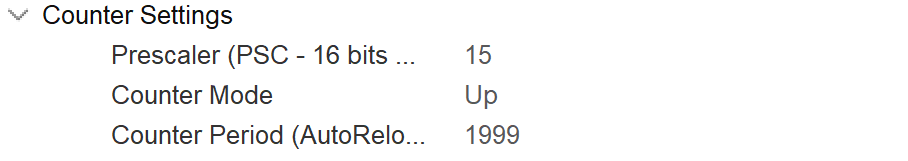
\includegraphics[width=0.9\linewidth]{assets/10.png}
        \caption{TIM3设置}
    \end{minipage}
    \begin{minipage}{0.49\textwidth}
        $$
        t=\frac1{48\cdot10^6}\cdot(16-1)=1/3us
        $$
    \end{minipage}
\end{figure}
TIM3中断控制代码:\par
\begin{lstlisting}[language=c]
if(LL_TIM_IsActiveFlag_UPDATE(TIM3)!= RESET)
{
    LL_TIM_ClearFlag_UPDATE(TIM3);
    renew(timecount%240,idx_c); //调用LED显示函数
    timecount++;    //计数
}
\end{lstlisting}
\section{程序编写过程}
\subsection{程序流程设计}
程序大致流程图如下所示:
\begin{figure}[H]
    \centering
    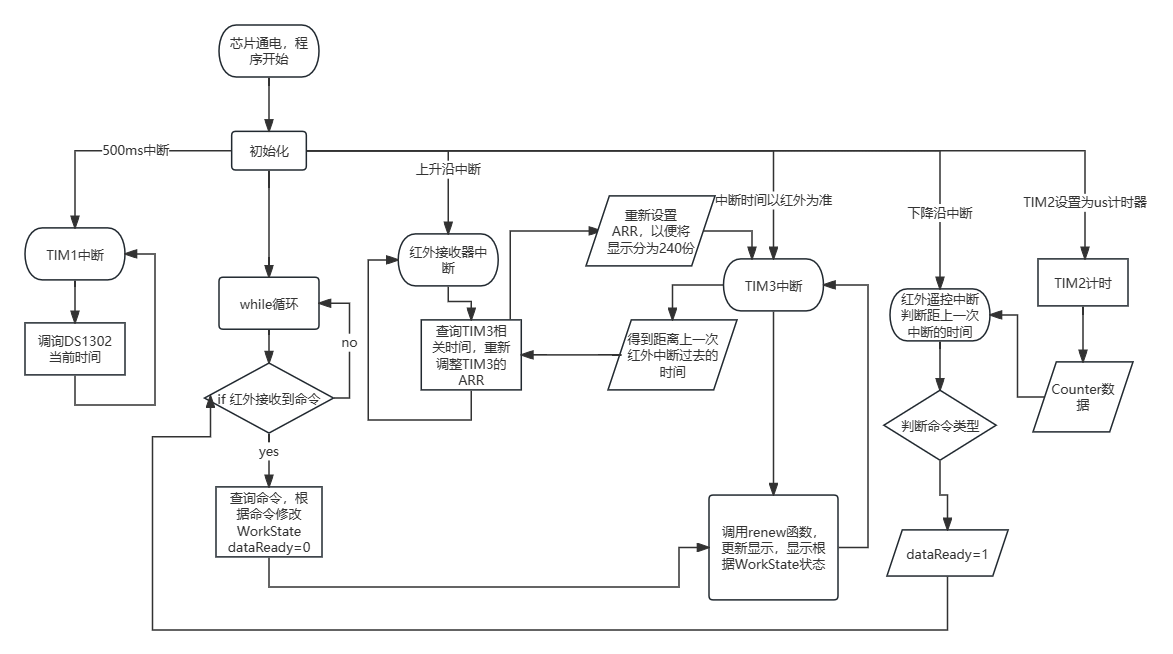
\includegraphics[width=0.9\linewidth]{assets/未命名文件.png}
    \caption{程序流程图}
\end{figure}
\subsection{软件功能细节部分实现}
\subsubsection{坐标转换}
64*64xy轴坐标变换为240*32的极坐标,并交给LED然后显示。在程序外编写一个坐标转换函数,然后将结果输出,使得能够在STM32中使用:
\begin{multicols}{2}
\begin{lstlisting}[language=c]
void polar_transform(unsigned char polar_bitmap[4][ANGLES][RADIUS]) {
    int cx = WIDTH / 2;
    int cy = HEIGHT / 2;
    for (int w = 0; w < 4; w++)
    {
        for (int angle = 0; angle < ANGLES; angle++) {
            double theta = (2.0 * M_PI * angle) / ANGLES;
            
            for (int r = 0; r < RADIUS; r++) {
                int x = cx + (int)(r * cos(theta));
                int y = cy - (int)(r * sin(theta));
                
                if (x >= 0 && x < WIDTH && y >= 0 && y < HEIGHT) {
                    int byte_index = (y * WIDTH + x) / 8;
                    int bit_index = 7 - ((y * WIDTH + x) % 8);
                    int pixel_value = (bitmap_bytes[w][byte_index] >> bit_index) & 0x01;
                    
                    polar_bitmap[w][angle][r] = pixel_value;
                } else {
                    polar_bitmap[w][angle][r] = 0;
                }
            }
        }
    }
}
\end{lstlisting}
\end{multicols}
\subsubsection{LED显示renew()函数}
LED显示数据
\begin{multicols}{2}
\begin{lstlisting}[language=c]
void renew(uint8_t idx_datab,uint8_t idx_datac)
{
  uint32_t tmp=0x80000000;  //595芯片显示掩码
  uint32_t shine=datac_pre[idx_datac]<<16;  
  uint8_t spointer,mpointer,hpointer;
  if((WorkState&NEC_Show)==0)
  {
    /*时钟指针的相关代码*/
    shine|=datab_pre[idx_datab];
    /*将s,m,h转换为转盘上240刻度的对应位置*/
    spointer=spoint*4;
    mpointer=spointer/60+mpoint*4;
    hpointer=mpointer/12+hpoint*20;
    shine|=display_date(idx_datab);
    if(idx_datab==(239-spointer)) shine|=0xF0FF;
    else if(idx_datab==(239-mpointer))  shine|=0xFC; 
  }
  else
  {
    show_cnt++; //动画切换帧
    if(show_cnt>=480)
    {
      show_cnt=0;
      show_flag=(show_flag+1)%4;
    }
    shine |= x[show_flag][idx_datab];
  }
  /*595芯片显示,代码在上已显示,具体略*/
  if((WorkState&NEC_Show)==0)   //相关WorkState状态为0
  {
    /*设置GPIO显示时钟*/
  }
  else  //相关WorkState状态为1
  {
    /*显示预设置动画*/
    tmp=y[show_flag][idx_datab]&0xFF;
    LL_GPIO_ResetOutputPin(GPIOA,tmp);
    tmp^=0xFF;
    LL_GPIO_SetOutputPin(GPIOA,tmp);
    tmp=((y[show_flag][idx_datab]>>8)&0x7)|((y[show_flag][idx_datab]>>1)&0x7C00);
    LL_GPIO_ResetOutputPin(GPIOB,tmp);
    tmp^=0x7C07;
    LL_GPIO_SetOutputPin(GPIOB,tmp);
  }
}
\end{lstlisting}
\end{multicols}
\paragraph{代码说明}
\begin{itemize}
    \item $\texttt{idx\_datab}$为转盘上当前显示的数据,$\texttt{idx\_datac}$为侧边当前显示的数据的位置,由于侧边会转动,因此两个索引不同,使得两者显示分离。
    \item 先调用595相关显示,再调用$\texttt{LL\_GPIO}$相关显示,原因为595芯片显示速度较慢,需要先显示,否则显示有所扭曲。
    \item 实验中一开始创建动画数据x[4][240],y[4][240],结果显示内存不足。后在命名时将其定义为常量$\texttt{const}$,内存足量,应为将数据从RAM中移动到ROM中,减少了RAM的使用。
\end{itemize}
\section{最终实验结果}
\paragraph{实现功能}
\begin{itemize}
    \item 基础功能
    \begin{itemize}
        \item 侧边字幕旋转
        \item 上面表盘实时转动
    \end{itemize}
    \item 红外遥控器操纵,接收到红外遥控信号,上下红灯闪烁一次。
    \begin{itemize}
        \item CH键,切换显示时钟/动画
        \item >>键,侧边字幕右旋,多次点按,旋转速度不同
        \item <<键,侧边字幕左旋,多次点按,旋转速度不同
        \item 播放键,上下红灯开启/关闭
    \end{itemize}
\end{itemize}
\end{document}